\hsection{}%
\hsection{Introduction}%
%
Today, algorithms influence a bigger and bigger part of both of our daily private and work life.
They suggest interesting movies for us to watch or products to purchase.
They help us find efficient routes when driving by car or match us to the next available and sufficiently nearby taxi.
They control advertisement campaigns and suggest product pricing policies~\cite{MAM2021TROAIRWAFRAMG}.
They support us by suggesting good decisions in a variety of fields, ranging from engineering, timetabling and scheduling, product design, to logistic planning.
They will be the most important element of the transition of our industry to smarter manufacturing and intelligent production, where they can automate a variety of tasks, as illustrated in \cref{fig:intelligent_manufacturing}.

\begin{figure}%
\centering%
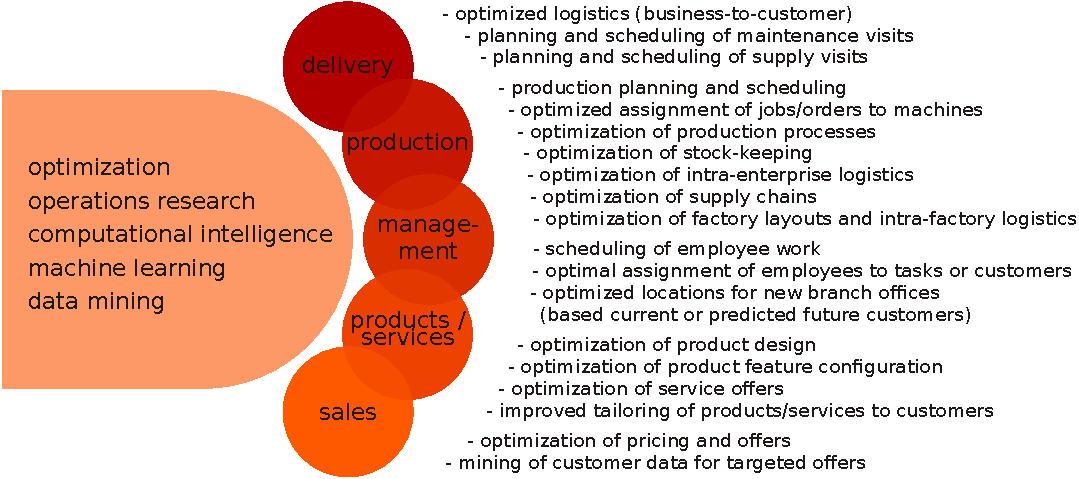
\includegraphics[width=0.99\linewidth]{\currentDir/intelligent_manufacturing}%
\caption{%
Examples for applications of optimization, computational intelligence, machine learning techniques in five fields of smart manufacturing: the production itself, the delivery of the products, the management of the production, the products and services, and the sales level.}%
\label{fig:intelligent_manufacturing}%
\end{figure}%

Optimization and Operations Research provide us with algorithms that propose good solutions to a very wide range of questions.
These solutions achieve a predefined goal while minimizing (at least) one resource requirement, be it costs, energy consumption, space, the time requirement, and so on.
Besides saving direct costs, the reduction of resource consumption often is also good for the environment.
Therefore, optimization can help us to become more efficient both economically and ecologically.

We can thus already list three obvious reasons why optimization will be a key technology for the next century:%
%
\begin{enumerate}%
%
\item The automation of production can improve the work life by reducing manual work while increasing productivity and product quality.
However, any form of intelligent production or smart manufacturing needs automated decisions.
Since these decisions should be \emph{intelligent,} they can only come from a process which involves optimization in one way or another.%
%
\item All branches of industry, all service sectors, as well as cities and regions face both global and local competition.
Those who can reduce their resource consumption and costs while improving product, production, or service quality and efficiency will have the edge.
One key technology for achieving this is better planning via optimization.%
%
\item Our world suffers from both depleting resources and too much pollution.
Optimization can \inQuotes{give us more while needing less.}
This often leads to more environmentally friendly processes.%
%
\end{enumerate}%
%
But how can algorithms help us to find solutions for hard problems in a variety of different fields?
How general are these algorithms?
How can they help us to make good decisions?
How can they help us to save resources?

In this book, we will try to answer all of these questions.
We will explore quite a lot of different optimization algorithms.
We will look at their actual implementations and we will apply them to example problems to see what their strengths and weaknesses are.%
%
\hinput{examples}{examples.tex}%
\hinput{metaheuristics}{metaheuristics.tex}%
%
\endhsection\endhsection%
%
